%!TEX root = ../masters_thesis.tex

\section{Hivent Model} % (fold)
\label{sec:hivent_model}

This section introduces the data model that represents countries and their evolution in time and space. In section \ref{sec:spatio_temporal_data_models}, different spatio-temporal data models were introduced to solve this problem. The \emph{Snapshot Model} is unsuitable for the problem space. \emph{Simple Time-Stamping} is helpful to link countries to their history, but it does not explicitly model historical changes, which is desireable. For that purpose, the idea of the \emph{Event-Based Spatio-Temporal Data Model} was developed, but since it only works for raster data, it is also not suitable for this thesis. This problem is solved in the \emph{History Graph Model}. Additionally, the introduced temporal changes allow to represent historical changes and their influences on geographic entities directly in the model. Finally, the \emph{Three-Domain Model} introduces a helpful concept to separate the spatial, temporal and thematic dimension of a spatio-temporal entity.

The \emph{Hivent Model} is constructed from components of some of these models: An Event-Based Spatio-Temporal Data Model supporting vector data. It is organized according to the Three-Domain Model and allows to visualize the evolution on a History Graph. In the first section of this section, the main elements of the Hivent model are introduced. Afterwards, the preconditions are defined. Finally, the Historical Geographic Operations that describe changes of countries in time and space are explained.

% ------------------------------------------------------------------------------
\subsection{Elements} % (fold)
\label{sub:elements}

The main elements of the the model are \emph{Hivent}s, representing an historically significant happening and \emph{Area}s, an abstract entity on a map with a name and a territory. An \emph{Historical Change} is part of one Hivent and manipulates the history of one or more Areas.

% - - - - - - - - - - - - - - - - - - - - - - - - - - - - - - - - - - - - - - -
\vspace{-1em}
\paragraph{Hivents} % (fold)
\label{par:hivent}

are the main organizing elements of the data model. The word is an acronym for \emph{\textbf{Hi}}storical e\emph{\textbf{vent}}. It represents a significant happening in history, e.g. a treaty, bill or declaration. The focus in this work is on events that influence the geopolitical situation on Earth. An Hivent happens at one particular point in time and space and introduces historical changes to countries.

% paragraph hivent (end)

% - - - - - - - - - - - - - - - - - - - - - - - - - - - - - - - - - - - - - - -
\vspace{-1em}
\paragraph{Areas} % (fold)
\label{par:area}

represent one identical current or historical country with a \emph{name} and a \emph{territory} on the map. The name of the Area consists of a common \emph{short name}, e.g. ``Germany'' and a \emph{formal name}, e.g. ``Federal Republic of Germany''. The \emph{territory} of the Area is described by a polypolygon, a set of weakly simple polygons to support enclaves and exclaves. The polylines of the polygons consist of an ordered set of points that represent the country border. The borders of a country are either \emph{interior}, i.e. bordering another country, or a \emph{coastline}, bordering a body of water. Additionally, each Area is keeps references to the \emph{start change} and \emph{end change}, the historical changes that created or ceased the Area, and to all \emph{update changes} that change the territory and name of the Area.

% paragraph area (end)

% ------------------------------------------------------------------------------
\vspace{-1em}
\paragraph{Historical Changes} % (fold)
\label{par:historical_changes}

influence the development of an Area over time. Throughout the lifetime of an Area, it is created at some point $t_s$, then its territory and short name can change multiple times $t_i: t_s < t_i$ and at some point $t_e: t_s < t_i < t_e$ it ceases. Since all changes in this model are sudden, there are only two possible states an Area can be in: It is \emph{active}, if at the current time point it is historically existing and it is \emph{inactive} if it does not. Each area is uniquely identified by its formal name. That means, the short name can change, but as soon as the formal name of an area changes (e.g. ``German Empire'' to ``Federal Republic of Germany''), it is considered a ``new'' Area.

Each Historical Change belongs to exactly one Hivent, inheriting its time point at which the change happens.  The change is described by a Historical Geographic Operation introduced in section \ref{sub:historical_geographic_operations}.

\begin{figure}[H]
  \vspace{1em}
  \centering
  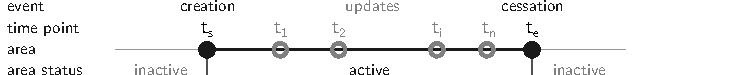
\includegraphics[width=0.9\textwidth]{graphics/development/area_states}
  \caption{Three event types that change Areas, resulting in two different area states}
  \label{fig:area_states}
\end{figure}


% paragraph historical_changes (end)

% subsection section area (end)

% ------------------------------------------------------------------------------
\subsection{Preconditions} % (fold)
\label{sub:preconditions}

\begin{quoteit}
In the beginning God created the heavens and the Earth \\
Now the Earth was formless and empty [...] \\
And God said, “Let there be light” --- and there was light.
\end{quoteit}
\hfill -- Genesis 1:1, The First Book of Moses, Old Testament

There are five axoims and two assumptions that are the basis of the spatio-temporal system developed in this thesis. The theoretical foundation is the model of the Earth, its curved surface that can be projected on a two-dimensional map using a map projection, as introduced in sections \ref{sub:model_of_geographical_space} and \ref{sub:presentation_of_geographic_space}.

\vspace{-1.0em}
\newtheorem{invariant_surface}[assicounter]{Axiom}
\begin{invariant_surface}
\label{axm:invariant_surface}
  The Earth's surface has an invariant area size, i.e. it does not change over time.
\end{invariant_surface}

\vspace{-2.5em}
\newtheorem{area_on_surface}[assicounter]{Axiom}
\begin{area_on_surface}
\label{axm:area_on_surface}
  Each Area in the spatio-temporal system is located directly on the surface of the Earth.
\end{area_on_surface}

These axiom sets the spatial foundation of the system: a constant dimension of the map and Areas covering the map. The basis of the temporal part of the system is content of the next three axioms:

\vspace{-1.0em}
\newtheorem{initial_configuration}[assicounter]{Axiom}
\begin{initial_configuration}
\label{axm:initial_configuration}
  The spatio-temporal system has an initial state at time point $t_0$. At this initial state, there exists exactly one Area, denoted by $\Omega$ and referred to as the \emph{universe} Area. It has no name and its territory covers the whole surface of the Earth.
\end{initial_configuration}

\vspace{-2.5em}
\newtheorem{historical_change}[assicounter]{Axiom}
\begin{historical_change}
\label{axm:historical_change}
  At each time point $t_i \geq t_0$ an Historical Change can be introduced.
\end{historical_change}

\vspace{-2.5em}
\newtheorem{unique_coverage}[assicounter]{Axiom}
\begin{unique_coverage}
\label{axm:unique_coverage}
  At each time point $t_i \geq t_0$ each point on the surface of the Earth is covered by exactly one territory of exactly one Area.
\end{unique_coverage}

As it has been defined in section \ref{par:historical_changes}, an Historical Change can create, manipulate and cease Areas on the Earth's surface. According to axoim \ref{axm:unique_coverage}, each change introduced in the system must maintain the spatial integrity on the map: When an Area with a territory is created on the map, the Area claiming this territory before has to cease this territory. Formally, it can be said that each change consists of a set of old Areas $A$ that are manipulated, a set of new Areas $B$ that are created in the change, and an operation $\rightarrow_C$ describing the change. Each Area $A_i \in A$ and $B_i \in B$ has a territory $A_i^T$  respectively $B_i^T$. For each change introduced in the system, the territories of the old Areas must have the same size than the territories of the new Areas to maintain the spatial integrity of axiom \ref{axm:unique_coverage}:
\begin{align}
  \bigcup\limits_{i=1}^n A_i^T ~\textbf{=}~ \bigcup\limits_{i=1}^n B_i^T
\end{align}

The first Historical Changes introduced in the system at time point $t_0$ are the creation of all bodies of water, including the oceans and lakes, denoted as $W$. Each Area $W_i \in W$ is created with their name and territory cut out of $\Omega$. The result is that at $t_0$, the map is divided into water ($W$) and land ($\Omega$). Land can at any point in time be either \emph{claimed}, i.e. it is currently occupied by the territory of exactly one active Area, or on a contrary be \emph{unclaimed}, i.e. belonging to $\Omega$. It is a subtractive data model, because each new Areas territory is cut out of $\Omega$.

\begin{figure}[H]
  \centering
  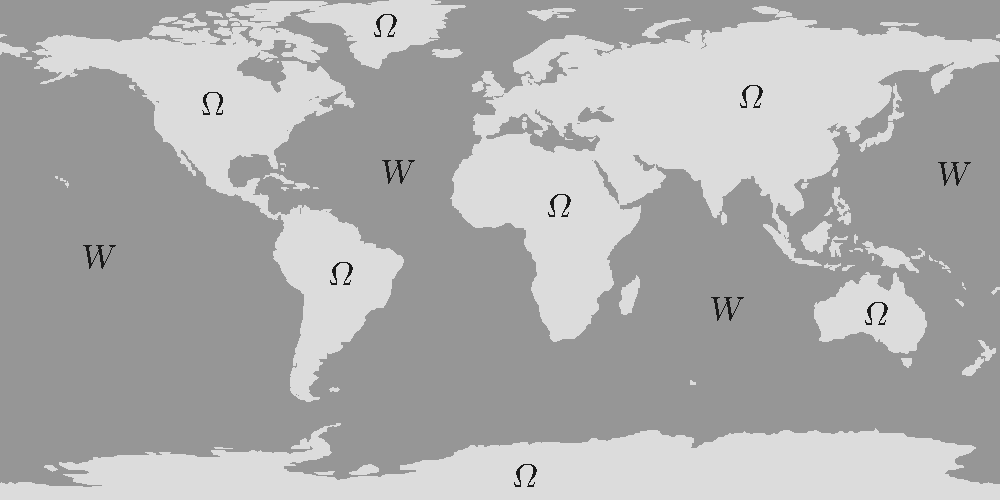
\includegraphics[width=0.5\textwidth]{graphics/development/init_map}
  \caption{The initial state of the world map at time point $t_0$}
  \label{fig:init_map}
\end{figure}

In the real world, the name of a country changes according to sudden events, e.g. a declaration or a governmental bill. The territory can change either because of a geographical processes, e.g. the sea level rise influencing the change of the coastline, or according to a historical event, e.g. a treaty. The Hivent model is based on two assumptions that simplify the model and keep the problem space clear:

\vspace{-1.0em}
\newtheorem{coastline_territory}[assicounter]{Assumption}
\begin{coastline_territory}
\label{axm:coastline_territory}
  The territory of a country stops at the coastline.
\end{coastline_territory}

\vspace{-1.5em}
\newtheorem{constant_coastlines}[assicounter]{Assumption}
\begin{constant_coastlines}
\label{axm:constant_coastlines}
  The spatial configuration of the Earth's surface, i.e. land, water and the coastlines, has not changed over time.
\end{constant_coastlines}

Both assumptions are obviously wrong: In line with \cite{UNSeaBorders}, the territory of a country extends in a range of 3 to 12 miles (5 to 20 kilometers) into international waters. They are constantly changing and so does the distribution of land and water on Earth. However, the assumptions allow the Hivent Model to focus only on discrete historical changes and not on long-term processes. In this data model, the temporal behavior of an Area can therefore be described as a \emph{static object that changes according to sudden events}.

% base: Newtons concept of absolute space?
% TODO: topological rule?
% each border has exactly two neighboring Areas
% each Area has at least one neighboring Area

% subsection preconditions (end)

% ------------------------------------------------------------------------------
\subsection{Historical Geographic Operations} % (fold)
\label{sub:historical_geographic_operations}

Respecting the preconditions, there are several different types of changes that can occur to a set of Areas. All possible changes can be expressed with only five spatio-temporal operations that are called \emph{Historical Geographic Operations} (HG Operations). The first four change the identity of a set of Areas and therefore establish historical predecessor-successor-relationships. They are always symmetric, i.e. if one old Area is replaced by one new Area, the old Area is the historical predecessor of the new Area and vice versa the new Area is the successor of the old Area.

\begin{description}
  \item[UNI -- Unification]
  A set of old Areas unifies to one new Area. The old Areas cease, becoming the historical predecessors of the new Area. This new Area receives a new name and its territory is the union of the territories of the old Areas. \\[0.25em]
  \begin{footnotesize}
    In 1922, the Russian SFSR, the Transcaucasian SFSR, the Ukrainian SSR and the Byelorussian SSR unified and formed the Union of Soviet Socialist Republics (USSR).
  \end{footnotesize}
  \item[INC -- Incorporation]
  One or more old Areas are incorporated into another Area that stays active. Its territory is enlarged by the union of the territories of the old Areas. The old Areas are historical predecessors of the new Area. \\[0.25em]
  \begin{footnotesize}
    In 1990, the territory of the German Democratic Republic (East Germany) became part of the Federal Republic of Germany (West Germany). Although this event is known as the \emph{German Reunification}, it is historically an incorporation of East Germany into West Germany \cite{incorporationEastWestGermany}.
  \end{footnotesize}
  \item[SEP -- Separation]
  As the inverse of unification, one old Area is preceded by multiple new Areas. Each new Area gets a new name, receives a part of the territory of the old Area, and the old Area as its only historical predecessor. \\[0.25em]
  \begin{footnotesize}
    In 1993, the Czech and Slovak Federal Republic, commonly known as Czechoslovakia, dissolved into present-day Czech Republic and Solvak Republic, creating two new countries out of one old.
  \end{footnotesize}
  \item[SEC -- Secession]
  As the inverse of incorporation, one or more new areas are ceded from a previously exising area that stays active. Each new Area gets a new name, receives the previously existing Area as the only historical predecessor and a part of its territory. \\[0.25em]
  \begin{footnotesize}
    In 2008, the Republic of Kosovo declared independence from Serbia and has since then partially received international recognition. Unlike in the case of separation, Serbia stays as country, keeping its name, but ceding a part of its territory to Kosovo.
  \end{footnotesize}
  \item[NCH -- Name Change]
  An Area changes its short name but preserves its identity. \\[0.25em]
  \begin{footnotesize}
    A recent change happened on 5. May 2016: The cabinet of Czech Republic approved that the country will now offically be called ``Czechia''. However, the formal name stays ``Czech Republic'', which preserves its identity.
  \end{footnotesize}
\end{description}

HG Operations can be combined when they happen at the same time, e.g. if one Area incorporates another Area and thereby changes its short name, this is a combination of \texttt{INC + NCH}. When West Germany incorporated East Germany in 1900, it was from that moment on just called Germany.

% - - - - - - - - - - - - - - - - - - - - - - - - - - - - - - - - - - - - - - -
\begin{table}[H]
\begin{center}
\begin{tabular}{m{0.75cm} m{2.5cm} m{2.5cm} cx{2.5cm}}
  \toprule
  & operation
  & \multicolumn{1}{c}{visualization}
  & \multicolumn{1}{c}{\pbox{2.5cm}{historical\\relationship\protect\footnotemark}} \\

  \midrule
  \texttt{UNI} & Unification & \raisebox{-0.25\height}
  {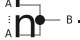
\includegraphics{graphics/development/hg_operations/UNI}} &
  $ A_i \leftrightarrow_H B_1 $ \\

  \midrule
  \texttt{INC} & Incorporation & \raisebox{-0.25\height}
  {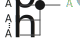
\includegraphics{graphics/development/hg_operations/INC}} &
  $ A_i \leftrightarrow_H A_0 $ \\

  \midrule
  \texttt{SEP} & Separation & \raisebox{-0.25\height}
  {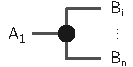
\includegraphics{graphics/development/hg_operations/SEP}} &
  $ A_1 \leftrightarrow_H B_i $ \\

  \midrule
  \texttt{SEC} & Secession & \raisebox{-0.25\height}
  {
\includegraphics{graphics/development/hg_operations/SEC}} &
  $ A_0 \leftrightarrow_H B_i $ \\

  \midrule
  \texttt{NCH} & Name Change & \raisebox{-0.25\height}
  {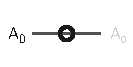
\includegraphics{graphics/development/hg_operations/NCH}} &
  $ \emptyset $ \\

  \bottomrule
\end{tabular}
\caption{The five HG Operations}
\label{tab:historical_geographic_operations}
\end{center}
\end{table}

\footnotetext{$A_i \leftrightarrow_H B_i$ denotes: $\forall i \in [1..n]:$ $A_i$ is historical predecessor of $B_i$ and $B_i$ is successor of $A_i$}

% subsection historical_geographic_operations (end)

% ------------------------------------------------------------------------------
\subsection{Edit Operations} % (fold)
\label{sub:edit_operations}

The Historical Geographic Operations are a valuable set of tools to describe all kinds of changes in the evolution of countries in time and space. They are really well understood from the system point of view and are therefore the basis for the Hivent Model. However, the purpose of the HGIS developed in this thesis is to provide an interface for the user to introduce historical changes to countries on the map.

Throughout the development process, interviews with historians and other researchers in humanities at University of Virginia were conducted, to understand their mental model about historical changes of countries. In the interviews it turned out that the HG Operations are not suitable to be used for human edit purposes, because of their low-level nature. One example is that the operations do not provide a straightforward way to create a new country on previously unclaimed land. The same is true for changing the formal name of an Area.

Therefore, this thesis introduces a second set of high-level operations to introduce changes to countries on the map: the \emph{Edit Operations} in table \ref{tab:edit_operations} have proven to be understandable in several user studies.

\begin{table}[H]
\begin{center}
\begin{tabular}{m{0.75cm} m{0.8cm} m{2.4cm} m{9.1cm}}
  \raisebox{-0.35\height}
  {
\includegraphics[width=0.72cm]{graphics/development/edit_operations/CRE}} &
  \texttt{CRE} & Create &
  a new Area with a new name and territory on the map. \\

  \raisebox{-0.35\height}
  {
\includegraphics[width=0.72cm]{graphics/development/edit_operations/MRG}} &
  \texttt{MRG} & Merge &
  two or more Areas to a new Area. The name has to be set manually, the territory is automatically unified. \\

  \raisebox{-0.35\height}
  {
\includegraphics[width=0.72cm]{graphics/development/edit_operations/DIS}} &
  \texttt{DIS} & Dissolve &
  one Area into two or more new Areas, manually setting their new territory and name. \\

  \raisebox{-0.35\height}
  {
\includegraphics[width=0.72cm]{graphics/development/edit_operations/CHB}} &
  \texttt{CHB} & Change Borders &
  between two neighboring Areas by defining the territory that changes sides. \\

  \raisebox{-0.35\height}
  {
\includegraphics[width=0.72cm]{graphics/development/edit_operations/REN}} &
  \texttt{REN} & Rename &
  an Area and set a new formal name, short name or both. \\

  \vspace{0.35em}
  \raisebox{-0.35\height}
  {
\includegraphics[width=0.72cm]{graphics/development/edit_operations/CES}} &
  \texttt{CES} & Cease &
  an Area by deleting it from the map, leaving unclaimed land. \\

\end{tabular}
\caption{The six Edit Operations}
\label{tab:edit_operations}
\end{center}
\end{table}


% subsection edit_operations (end)

% section hivent_model (end)